\begin{figure}[H]
\centering
%
\begin{subfigure}{0.31\textwidth}
  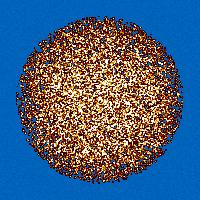
\includegraphics[width=0.9\linewidth]{figures/burn-20-bstep0}
  \caption{Fresh}
  \label{fig:bstep0}
\end{subfigure}%
%
\begin{subfigure}{0.31\textwidth}
  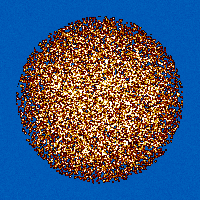
\includegraphics[width=0.9\linewidth]{figures/burn-20-bstep1}
  \caption{Six Months}
  \label{fig:bstep1}
\end{subfigure}%

\caption[Serpent-Generated Mesh Figures of the Fission Rate and Thermal Flux for the Representative Single-Pebble at each Depletion Step]{Serpent-generated mesh figures of the fission rate (hot color map) and thermal flux (cold color map) for the representative single-pebble at each depletion step.  A cold color map is from shades of whitish-blue (high) to blackish-blue (low) while the hot color map is from a whitish-yellow (high) to reddish-brown (low)}
\end{figure}

\begin{figure}[H]\ContinuedFloat
\centering

\begin{subfigure}{0.31\textwidth}
  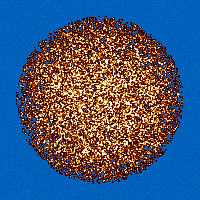
\includegraphics[width=0.9\linewidth]{figures/burn-20-bstep2}
  \caption{Twelve Months}
  \label{fig:bstep2}
\end{subfigure}%
%
\begin{subfigure}{0.31\textwidth}
  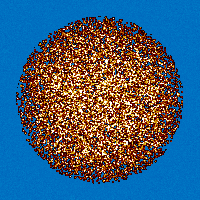
\includegraphics[width=0.9\linewidth]{figures/burn-20-bstep3}
  \caption{Eighteen Months}
  \label{fig:bstep3}
\end{subfigure}%

\begin{subfigure}{0.31\textwidth}
  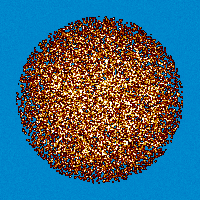
\includegraphics[width=0.9\linewidth]{figures/burn-20-bstep4}
  \caption{Twenty-Four Months}
  \label{fig:bstep4}
\end{subfigure}%
%
\begin{subfigure}{0.31\textwidth}
  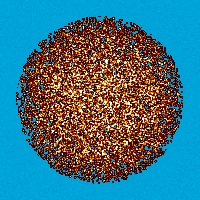
\includegraphics[width=0.9\linewidth]{figures/burn-20-bstep5}
  \caption{Thirty Months}
  \label{fig:bstep5}
\end{subfigure}%

\begin{subfigure}{0.31\textwidth}
  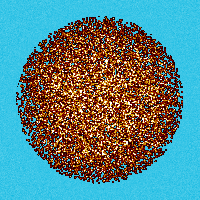
\includegraphics[width=0.9\linewidth]{figures/burn-20-bstep6}
  \caption{Thirty-Six Months}
  \label{fig:bstep6}
\end{subfigure}%
%
\caption[]{(cont.)}
\label{fig:burn-meshes}
\end{figure}